\documentclass[11pt]{article}

\usepackage{fullpage}
\usepackage{rotating}   
\usepackage{amsmath}
\usepackage{amssymb}
\usepackage{amsthm}
\usepackage{fancyhdr}
\usepackage{algorithm}
\usepackage{algorithmic}
\usepackage{bm}
\usepackage{listings}
\usepackage{graphicx}
\usepackage{caption2}
\usepackage{subfigure}
\usepackage{float}
\usepackage{extpfeil}
\usepackage{color}
\usepackage[usenames,dvipsnames]{xcolor}


\newtheorem{theorem}{Theorem}[section]
\newtheorem{lemma}[theorem]{Lemma}
\newtheorem{corollary}[theorem]{Corollary}
\newtheorem{proposition}[theorem]{Proposition}
\newtheorem{definition}[theorem]{Definition}
\newtheorem{conjecture}[theorem]{Conjecture}
\newtheorem{remark}[subsection]{Remark}

%%
\newcommand\numberthis{\addtocounter{equation}{1}\tag{\theequation}}

%% define new symbols
\def\bx{\bm{x}}
\def\bb{\bm{b}}
\def\ba{\bm{a}}
\def\bc{\bm{c}}
\def\bf{\bm{f}}
\def\by{\bm{y}}
\def\bu{\bm{u}}
\def\bv{\bm{v}}
\def\BW{\bm{W}}
\def\BA{\bm{A}}
\def\bz{\bm{z}}
\def\BZ{\bm{Z}}
\def\BH{\bm{H}}
\def\BL{\bm{L}}
\def\BU{\bm{U}}
\def\BV{\bm{V}}
\def\BB{\bm{B}}
\def\BC{\bm{C}}
\def\BD{\bm{D}}
\def\BE{\bm{E}}
\def\BW{\bm{W}}
\def\BQ{\bm{Q}}
\def\BG{\bm{G}}
\def\BA{\bm{A}}
\def\BX{\bm{X}}
\def\BY{\bm{Y}}
\def\BQ{\bm{Q}}
\def\BI{\bm{I}}
\def\BR{\bm{R}}

%% define new brackets
\def\la{\left\langle}
\def\ra{\right\rangle}
\def\ln{\left\|}
\def\rn{\right\|}
\def\lb{\left(}
\def\rb{\right)}
\def\lsb{\left[}
\def\rsb{\right]}
\def\lcb{\left\{}
\def\rcb{\right\}}

%%
\DeclareMathOperator*{\argmin}{arg\,min}
\DeclareMathOperator*{\argmax}{arg\,max}

%%
\title{Homework VIII}
\author{Name: Shao Yanjun, Number: 19307110036}


\begin{document}
\maketitle

%------------------------------------
\begin{abstract}
This is Daniel's homework of  "Numerical Algorithms with Case Studies II".
\end{abstract}
%-------------------------------------
%=====================
\section{Problems}
\paragraph{Q1}
We will try $f(x)=p$, $f(x)=px+q$, $f(x)=px^2+qx+r$, etc.
\begin{align}
	&\int_{-2a}^{2a}p\mathrm{d}x=4ap=(c_1+c_2+c_3)p\\
	&\int_{-2a}^{2a}px+q\mathrm{d}x=4aq=-a(c_1-c_3)p+(c_1+c_2+c_3)q\\
	&\int_{-2a}^{2a}px^2+qx+r\mathrm{d}x=\frac{16}{3}a^3p+4ar=a^2(c_1+c_3)p-a(c_1-c_3)q+(c_1+c_2+c_3)r\\
	&\int_{-2a}^{2a}px^3+qx^2+rx+s\mathrm{d}x=\frac{16}{3}a^3q+4as=-a^3(c_1-c_3)p+a^2(c_1+c_3)q-a(c_1-c_3)r+(c_1+c_2+c_3)s
\end{align}
For higher degree polynomials, There couldn't be any solution for $c_1,c_2,c_3$. However, for $\mathbf{deg}p(x)=3$, we have $c_1=\dfrac{8}{3}a,c_2=-\dfrac{4}{3}a,c_3=\dfrac{8}{3}a$.
\paragraph{Q2}
\subparagraph{(a)}
I assert that the degree of exactness of this rule can't exceed the first order. We can check this assertion by examining its performance on quadratic integration and linear integration. For any linear function $f(x)=cx+d$,
\begin{align}
	\int_{a}^{b}f(x)\mathrm{d}x&=\frac{c}{2}(b^2-a^2)+d(b-a)=\frac{b-a}{2}(c(\frac{2a+b}{3}+\frac{a+2b}{3})+2d)\\&=\frac{b-a}{2}(f(\frac{2a+b}{3})+f(\frac{a+2b}{3}))
\end{align} 
The result is exact. However, for quadratic function $f(x)=(x-\frac{2a+b}{3})(x-\frac{a+2b}{3})$,
\begin{align}
	\int_{a}^{b}f(x)\mathrm{d}x&=\frac{1}{3}(b^3-a^3)-\frac{1}{2}(a+b)(a^2-b^2)+\frac{1}{9}(2a+b)(a+2b)(b-a)\\&\ne0=\frac{b-a}{2}(f(\frac{2a+b}{3})+f(\frac{a+2b}{3}))
\end{align}
This means at least for some quadratic functions, this rule can't reach exactness.
\subparagraph{(b)}
Directly calculate the error on $[x_i,x_i+h]$,
\begin{align}
	\int_{x_i}^{x_i+h}sin(x)\mathrm{d}x&-\frac{h}{2}(sin(x_i+\frac{h}{3})+sin(x_i+\frac{2h}{3}))=-cos(x_i+h)+cos(x_i)-\frac{h}{2}sin(x_i+\frac{h}{3})+\frac{h}{2}sin(x_i+\frac{2h}{3})\\
	&\xlongequal{Taylor}hsin(x_i)+\frac{h^2}{2}cos(x_i)-\frac{h^3}{6}sin(\xi)-\frac{h}{2}(sin(x_i)+\frac{h}{3}cos(x_i)-\frac{h^2}{18}sin(\eta_1))\\
	&+\frac{h}{2}(sin(x_i)+\frac{2h}{3}cos(x_i)-\frac{4h^2}{18}sin(\eta_2))\\
	&=O(h^3)
\end{align}
The error is $O(h^3)$ level.
\paragraph{Q3}
\subparagraph{(a)}
Let $h=\dfrac{b-a}{n}$, we can rewrite our estimation as follows,
\begin{align}
	\int_{a}^{b}f(x)\mathrm{d}x=\sum_{i=1}^{n}\int_{x_i}^{x_i+h}f(x)\mathrm{d}x\approx\sum_{i=1}^{n}f(x_i+\frac{h}{2})
\end{align}
Estimate the error with the help of Taylor theorem,
\begin{align}
	\int_{a}^{b}f(x)\mathrm{d}x-\sum_{i=1}^{n}f(x_i+\frac{h}{2})&=
	\sum_{i=1}^{n}\int_{x_i}^{x_i+h}f(x)-f(x_i+\frac{h}{2})\mathrm{d}x\\
	&=\sum_{i=1}^{n}\int_{x_i}^{x_i+h}(f(x_i+\frac{h}{2})+f'(x_i+\frac{h}{2})(x-(x_i+\frac{h}{2}))\\&+f''(\eta_i)(x-(x_i+\frac{h}{2}))^2-f(x_i+\frac{h}{2}))\mathrm{d}x\\
	&=\sum_{i=1}^{n}f''(\eta_i)\int_{-\frac{h}{2}}^{\frac{h}{2}}x^2\mathrm{d}x\\
	&\le \frac{nh^3}{24}f''(\eta_i)_{max}=\frac{(a-b)^3}{24n^2}f''(\eta_i)_{max}\\
\end{align}
Since $f : [a, b] \rightarrow \Re$ is twice continuously differentiable, $\exists\xi\in[a,b]$, s.t. $f''(\xi)=f''(\eta_i)_{max}$. Therefore, we have the truncation error following the upper bound.
\subparagraph{(b)}
Use the upper bound given by (a), we will be easy to calculate the smallest $n$ that meets the requirement.
\begin{align}
	\frac{1}{24n^2}f''(\xi)\le\frac{e}{24n^2}\le10^{-6}
\end{align}
\begin{figure}[H]
	\centering
	\subfigure[Converge to $\int_{0}^{1}e^x\mathrm{d}x$]{
		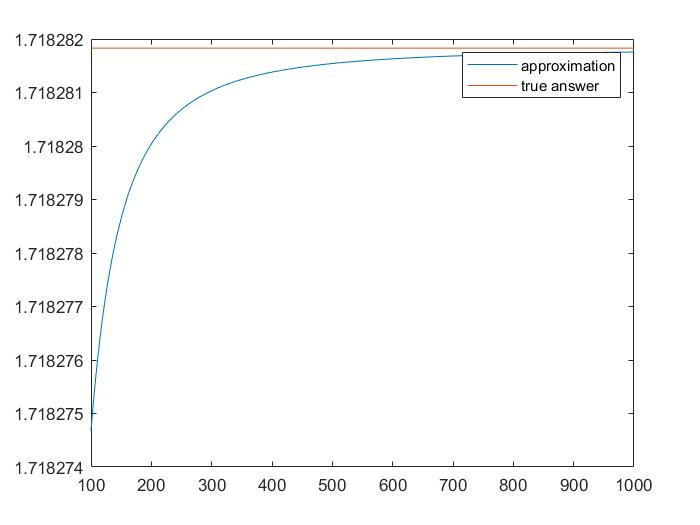
\includegraphics[width=0.6\linewidth]{convergence.jpg}
	}
\end{figure}
\paragraph{Q4}
Use Romberg method, we get $\int_{0}^{1}e^x \mathrm{d}x\approx1.71828$ and $\int_{0}^{1}x^{\frac{3}{2}}\mathrm{d}x\approx0.39999$.
\begin{figure}[H]
	\centering
	\subfigure[Converge to $\int_{0}^{1}e^x\mathrm{d}x$]{
		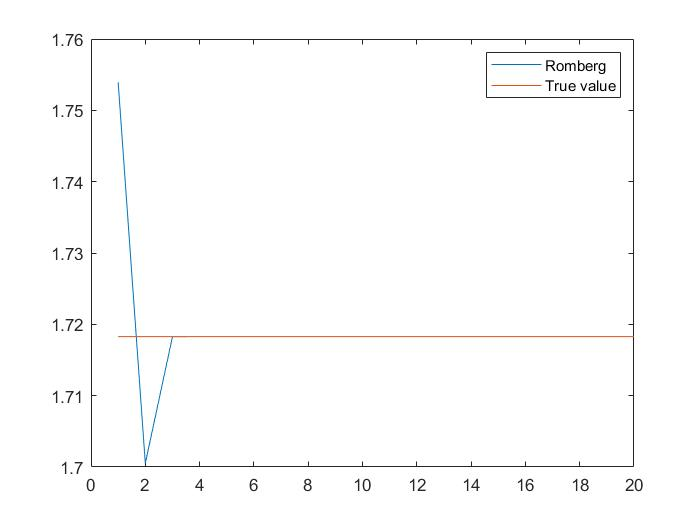
\includegraphics[width=0.4\linewidth]{convergence2.jpg}
	}
	\subfigure[Converge to $\int_{0}^{1}x^{\frac{3}{2}}\mathrm{d}x$]{
		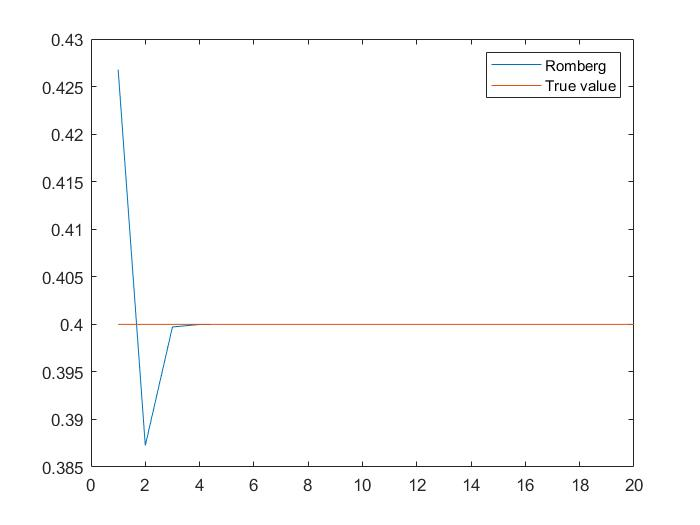
\includegraphics[width=0.4\linewidth]{convergence3.jpg}
	}
\end{figure}
The convergence routine seems similar.
\paragraph{Q5}
Use the parametric curve formula and calculate the circumference of an ellipse. Try Romberg method, the result converges to $L=4\int_{0}^{\frac{\pi}{2}}\sqrt{a^2cos^2(\theta)+b^2sin^2(\theta)}\mathrm{d}\theta\approx3.7822948\times10^8km$.
%-------------------------------------
%=====================
\end{document}
